%%%%%%%%%%%%%%%%%%%%%%%%%%%%%%%%%%%%%
% Document properties and packages
%%%%%%%%%%%%%%%%%%%%%%%%%%%%%%%%%%%%%
\documentclass[a4paper,12pt,final]{memoir}
\usepackage{CJKutf8}%中文支持

% misc
\renewcommand{\familydefault}{bch}	% font
\pagestyle{empty}					% no pagenumbering
\setlength{\parindent}{0pt}			% no paragraph indentation
% required packages (add your own)
\usepackage{flowfram}% column layou
\usepackage{marvosym}
\usepackage{textcomp}

\usepackage[top=1cm,left=1cm,right=1cm,bottom=1cm]{geometry}% margins
\usepackage{graphicx}										% figures
\usepackage{hyperref}
\definecolor{linkcolour}{rgb}{0,0.2,0.6}  %蓝色
\hypersetup{colorlinks,breaklinks,urlcolor=linkcolour, linkcolor=linkcolour}% URLs
\usepackage[usenames,dvipsnames]{xcolor}					% color
\usepackage{multicol}										% columns env.
	\setlength{\multicolsep}{0pt}
\usepackage{paralist}										% compact lists
\usepackage{tikz}

%%%%%%%%%%%%%%%%%%%%%%%%%%%%%%%%%%%%%
% Create column layout
%%%%%%%%%%%%%%%%%%%%%%%%%%%%%%%%%%%%%
% define length commands
\setlength{\vcolumnsep}{\baselineskip}
\setlength{\columnsep}{\vcolumnsep}
%定义主题颜色,可选颜色 Maroon,ForestGreen,DarkOrchid,RoyalBlue,Turquoise,Cyan,etc,更多颜色参考xcolor包的颜色定义
\newcommand{\myThemeColor}{RoyalBlue}
% frame setup (flowfram package)
% left frame
\newflowframe{0.23\textwidth}{\textheight}{0pt}{0pt}[left]
	\newlength{\LeftMainSep}
	\setlength{\LeftMainSep}{0.23\textwidth}
	\addtolength{\LeftMainSep}{1\columnsep}

% small static frame for the vertical line
\newstaticframe{1.5pt}{\textheight}{\LeftMainSep}{0pt}

% content of the static frame
\begin{staticcontents}{1} %绘制分割线,使用tikz包绘制。如需改变风格线样式,请参考tikz教程,对于新手,不建议修改。
\hfill
\tikz{%
	\draw[loosely dotted,color=\myThemeColor,line width=1.5pt,yshift=0]
	(0,0) -- (0,\textheight);}%
\hfill\mbox{}
\end{staticcontents}

% right frame
\addtolength{\LeftMainSep}{1.5pt}
\addtolength{\LeftMainSep}{1\columnsep}
\newflowframe{0.7\textwidth}{\textheight}{\LeftMainSep}{0pt}[main01]


%%%%%%%%%%%%%%%%%%%%%%%%%%%%%%%%%%%%%
% define macros (for convience)
%%%%%%%%%%%%%%%%%%%%%%%%%%%%%%%%%%%%%
\newcommand{\Sep}{\vspace{1em}}
\newcommand{\SmallSep}{\vspace{0.9em}}

\newenvironment{AboutMe}
	{\ignorespaces\textbf{\color{\myThemeColor} About me}}
	{\Sep\ignorespacesafterend}
%定义section	
\newcommand{\CVSection}[1]
	{\Large\textbf{#1}\par
	\vspace{0.2cm}\normalsize\normalfont}

\newcommand{\CVItem}[1]
	{\textbf{\color{\myThemeColor} #1}}


%%%%%%%%%%%%%%%%%%%%%%%%%%%%%%%%%%%%%
% Begin document
%%%%%%%%%%%%%%%%%%%%%%%%%%%%%%%%%%%%%
\begin{document}

\begin{CJK*}{UTF8}{gbsn}%选择字体,黑体
% Left frame 左边内容在此定义
%%%%%%%%%%%%%%%%%%%%
\begin{figure}
	\hfill
	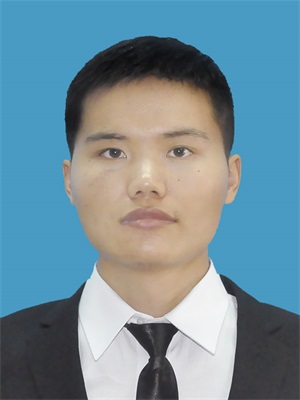
\includegraphics[width=0.8\columnwidth]{photo}
	\vspace{-7cm}
\end{figure}
\begin{flushright}\footnotesize
.\\
\vskip 6cm
    \raggedright
	\CVItem{{\large 个人信息:}}\\
\SmallSep
    出生年月:\\
    1991.8  \\
    \SmallSep
    联系电话:\\
	+86 - 1884262****  \\
\SmallSep
	电子邮件:\\
	\href{mailto:1150821146@qq.com}{1150821146@qq.com}  \\
\SmallSep
	个人博客:\\
	\href{https://echoorchid.github.io/}{https://echoorhid.github.io} \\
	
	\SmallSep
\SmallSep
\SmallSep
	\CVItem{{\large \\语言能力:}}\\

	\textit{\textbf{英语}:四六级~~~~511/476}\\
	\SmallSep
\SmallSep
\SmallSep
	\CVItem{{\large 电脑技能:}}\\
    \SmallSep
	$\bullet$\textbf{编程语言:}\\ C/C++, Matlab, Java, Python, Latex等\\
	\SmallSep
    $\bullet$\textbf{工作软件:}\\ Visual Studio, Matlab, Latex\\
	\SmallSep
	\textit{能够在Android和WP平台上编写简单的Apps,熟练使用\LaTeX 和LINUX}
	\SmallSep
\SmallSep
\SmallSep
	\CVItem{{\large 爱好:}}\\
\SmallSep
	\textit{慢跑,游泳,羽毛球,旅游 }
	\SmallSep
\end{flushright}\normalsize
\framebreak


% Right frame 右边内容在此定义
%%%%%%%%%%%%%%%%%%%%
\Huge\bfseries {\color{\myThemeColor} 胡~~卫~~东}\\
\normalsize\normalfont

% Education
\CVSection{教育背景}
\hrule
\SmallSep
\CVItem{2010.9 - 2014.6\hfill\textsc{大连理工大学~~~~学士学位}}\\
\textit{--电子信息工程}\\
\CVItem{2014.9 - 2017.6\hfill\textsc{大连理工大学~~~~硕士学位}}\\
\textit{--信息与通信工程}\\
\textit{--部分课程:C/C++入门 81、数字图像处理 89、面向对象编程技术 84. }

% Experience
\CVSection{专业技能}
\hrule
\SmallSep

\textit{$\bullet$ 熟练掌握 C/C++及面向对象编程思想。}

\textit{$\bullet$ 拥有丰富MFC 项目调试经验,熟悉图像处理,计算机视觉相关算法。}

\textit{$\bullet$ 了解 Git 语法、Git Hub 的开发流程,KeilC51 嵌入式软件开发。 }

\textit{$\bullet$ 国家英语四、六级,能很好阅读英文文献、说明书及开发文档手册。}

% CAMPU
\CVSection{专业经历}
\hrule
\SmallSep
\CVItem{2012.04 - 2013.03, 大学生创新项目(IPP)\hfill\emph{研究员}}\\
\textit{$\bullet$ 主导参加IPP项目,研究并可视化激光等离子体在真空环境下的聚焦点。}
\\
\CVItem{2013.05 - 2013.09, 大陆台湾能源合作\hfill\emph{研究专员}}\\
\textit{$\bullet$ 调研大陆能源供给和消费情况,相关资料提供给台湾学者使用,促进两岸科学交流}
\\
\CVItem{2013.02 - 2013.10, 奥迪绿色能源竞赛\hfill\emph{团队领导}}\\
\textit{$\bullet$ 领头参加绿色能源竞赛,我们的作品是“智能绿色候车公交站台”,并获一等奖}
\\
\CVItem{2012.06 - 2012.09, 社会实践\hfill\emph{团队领导}}\\
\textit{$\bullet$ 组织16个人的社会实践团队,深入甘肃会宁,为一个公益福利网站调查并收集贫困家庭信息,该项目获上海市社会实践优秀项目}

% HONORS & SCHOLARSHIPS
\CVSection{个人荣誉}
\hrule
\SmallSep
	\begin{tabular}{l|l}
		$\Rightarrow$ 2014.10&\textit{法国大使馆杰出人才奖学金}\footnotesize\\
		$\Rightarrow$ 2013.10&\textit{奥迪绿色能源竞赛一等奖}\\
		$\Rightarrow$ 2012.12&\textit{晨兴企业奖学金}\\
		$\Rightarrow$ 2012.10&\textit{连续三年获得上海交大优秀学生奖学金}\\
		$\Rightarrow$ 2011.04&\textit{上海市社会实践优秀项目}\footnotesize\\
	\end{tabular}

%%%%%%%%%%%%%%%%%%%%%%%%%%%%%%%%%%%%%
% End document
%%%%%%%%%%%%%%%%%%%%%%%%%%%%%%%%%%%%%
\end{CJK*}
\end{document}
